%%%%%%%%%%%%%%%%%%%% author.tex %%%%%%%%%%%%%%%%%%%%%%%%%%%%%%%%%%%
%
% sample root file for your "contribution" to a contributed volume
%
% Use this file as a template for your own input.
%
%%%%%%%%%%%%%%%% Springer %%%%%%%%%%%%%%%%%%%%%%%%%%%%%%%%%%%%%%%%%


% RECOMMENDED %%%%%%%%%%%%%%%%%%%%%%%%%%%%%%%%%%%%%%%%%%%%%%%%%%%
%\documentclass[graybox]{svmult}
%
%% choose options for [] as required from the list
%% in the Reference Guide
%
%\usepackage{mathptmx}       % selects Times Roman as basic font
%\usepackage{helvet}         % selects Helvetica as sans-serif font
%\usepackage{courier}        % selects Courier as typewriter font
%\usepackage{type1cm}        % activate if the above 3 fonts are
%                           % not available on your system
%
%\usepackage{makeidx}         % allows index generation
%\usepackage{graphicx}        % standard LaTeX graphics tool
%                             % when including figure files
%\usepackage{multicol}        % used for the two-column index
%\usepackage[bottom]{footmisc}% places footnotes at page bottom
%
%%custom package
%\usepackage{mathtools}
%\usepackage{cite}
%% see the list of further useful packages
%% in the Reference Guide
%
%\makeindex             % used for the subject index
%                       % please use the style svind.ist with
%                       % your makeindex program
%
%%%%%%%%%%%%%%%%%%%%%%%%%%%%%%%%%%%%%%%%%%%%%%%%%%%%%%%%%%%%%%%%%%%%%%%%%%%%%%%%%%%%%%%%%%%

%\begin{document}

\title{Global search algorithms for one-dimensional multiextremal optimization problems with nonlinear constraints}
% Use \titlerunning{Short Title} for an abbreviated version of
% your contribution title if the original one is too long
\author{Name of First Author and Name of Second Author}
% Use \authorrunning{Short Title} for an abbreviated version of
% your contribution title if the original one is too long
\institute{Name of First Author \at Name, Address of Institute, \email{name@email.address}
\and Name of Second Author \at Name, Address of Institute \email{name@email.address}}
%
% Use the package "url.sty" to avoid
% problems with special characters
% used in your e-mail or web address
%
\maketitle

\abstract{The chapter considers a method for reduction of a constrained problem to an
unconstrained one, so called \emph{index method}. This method, unlike the classical penalty function
one, allows avoiding the problem of the parameter selection (like the penalty coefficients for the
constraints) and also allows solving the problems with so called partially defined constraints,
which could not be solved by any other method. The serial and parallel algorithms for solving
univariate problems are considered.}

\keywords{multiextremal optimization, nonconvex constraints, index method, parallel
algorithms}

\section{Problem statement}
In the present chapter, the one-dimensional problems of the constrained optimization will
be considered. Let $\varphi(x)$ and $g_j(x)\le 0,1\le j\le m$, be the real functions defined in a closed interval $[a,b]$ of the real axis. It is requires to find the values $x^*$ satisfying the condition
\begin{equation}
  \label{eq4:problem}
  \varphi(x^*)=\min\{\varphi(x):x\in [a,b], g_j(x)\le 0,\; 1\le j\le m\}.
\end{equation}

As before, the objective function $\varphi$ (hereinafter denoted also as $g_{m+1}$) and the left parts of the constraints $g_j(x)\le 0,1\le j\le m$, are assumed to satisfy \emph{Lipschitz condition} with the corresponding constants $L_j,1\le j\le m+1$, namely:
\begin{equation}
  \label{eq4:lip_condition}
  |g_j(x_1)-g_j(x_2)|\le L_j|x_1-x_2|,1\le j\le m+1,x_1,x_2\in [a,b].
\end{equation}

\example{
\label{ex4:problem}
Let us consider a problem of type \eqref{eq4:problem} where $x\in [0.6,2.2],\; m=2$,
\begin{gather*}
  \varphi(x)=\cos(18x-3)\sin(10x-7)+1.5, \\
  g_1(x)=\exp(-x/2)\sin(6x-1.5), \\
  g_2(x)=|x|\sin(2\pi x-0.5).
\end{gather*}
The exact solution of the problem is $x^*=2.0795,\; \varphi(x^*)=0.565$. The graphs of the functions $g_1(x),g_2(x)$ and $\varphi(x)$ are presented in Fig. \ref{fig:4_1}.
\begin{figure}[ht]
  \centering
  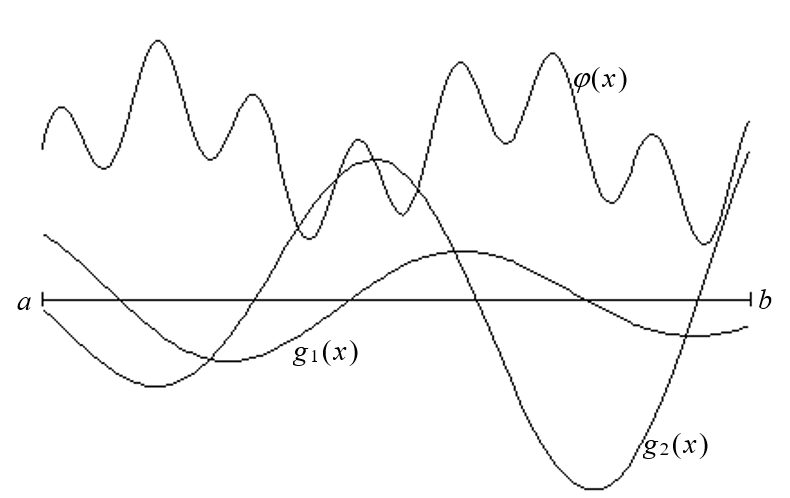
\includegraphics[width=0.8\textwidth]{figures/4_1.png}
  \caption{One-dimensional global optimization problem}
  \label{fig:4_1}
\end{figure}
}

\section{Partial computability and index scheme of the account of constraints}
Problem \eqref{eq4:problem} can be considered in the statement when each function $g_j,1\le j\le m+1$, is defined and computable only in the corresponding subdomains $Q_j\subset [a,b]$, where
\begin{equation}
  \label{eq4:q}
  Q_1=[a,b],Q_(j+1)=\{x\in Q_j:g_j(x)\le 0\},1\le j\le m.
\end{equation}

For example, in the optimal design problems some characteristics of the technical systems may appear to be undefined if the conditions of the system functioning represented by a part of the constraints of problem \eqref{eq4:problem} are not fulfilled.

Taking into account conditions \eqref{eq4:q}, initial problem \eqref{eq4:problem} can be represented in the form
\begin{equation}
  \label{eq4:problem2}
  \varphi(x^*)=\min\{g_{m+1}(x):x\in Q_{m+1}\}.
\end{equation}

For the purposes of further treatment, let us introduce a classification of the points $x$ in the search domain $[a,b]$ using an index $\nu=\nu(x)$ where $\nu-1$ is the number of constraints, which are fulfilled in this point. Formally, the index $\nu$ is defined by the conditions
\begin{equation}
  \label{eq4:condition}
  g_j(x)\le 0,\; 1\le j \le \nu-1,\; g_\nu(x)>0,
\end{equation}
(the last inequality is inessential  if $\nu=m+1$) and it satisfies the inequalities
\begin{displaymath}
  1\le\nu=\nu(x)\le m+1.
\end{displaymath}
The problem of example \ref{ex4:problem} assuming a partial computability of the functions is presented in Fig. \ref{fig:4_2}. The arcs of the restrictions $g_1(x),\:g_2(x)$, and of the objective function $\varphi(x)$ defined in the corresponding subdomains $Q_j$ from \eqref{eq4:q} are shown. The point $x^1$ with the index $\nu(x^1)=1$, the point $x^2$ with the index $\nu(x^2)=2$, and the point $x^3$ with the index $\nu(x^3)=3$ are shown also.

\begin{figure}[ht]
  \centering
  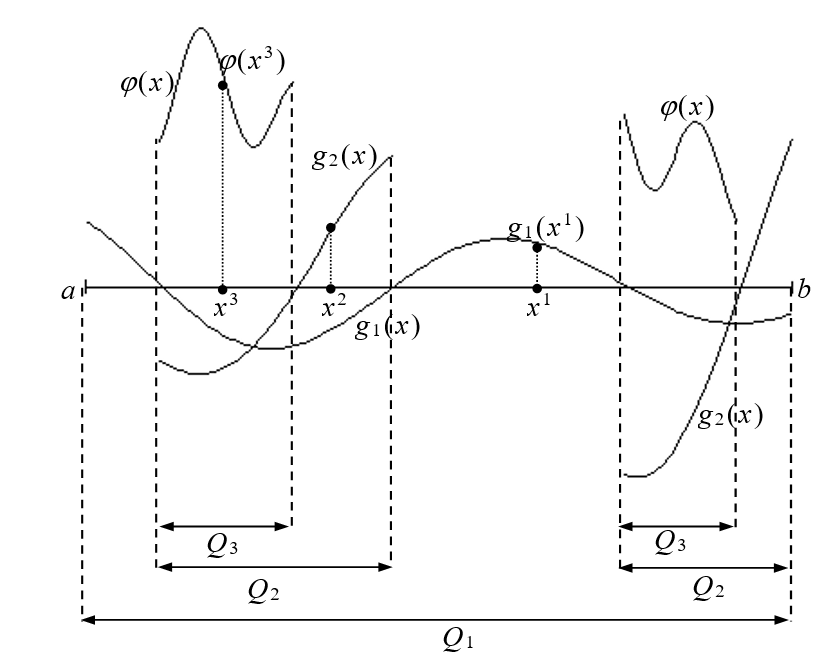
\includegraphics[width=0.8\textwidth]{figures/4_2.png}
  \caption{A problem with partially computable functions}
  \label{fig:4_2}
\end{figure}

This classification generates the function
\begin{equation}
  \label{eq4:fx}
  f(x)=g_\nu(x),\nu=\nu(x),
\end{equation}
defined and computable everywhere in $[a,b]$. Its value at a point $x$ is either the value of the left part of the constraint violated at this point (the case $\nu\le m$)  or the value of the objective function (the case $\nu=m+1$). Therefore, the determination of the value of $f(x),\:x\in[a,b]$  is reduced to a successive computations of the values of $g_j(x), 1\le j\le \nu=\nu(x)$, i.e., the next value $g_{j+1}(x)$ is calculated in the case when $g_j(x)\le 0$ only. The computational process finishes either as a result of the fulfillment of the inequality $g_j(x)>0$ or as a result of achievement of the value $\nu(x)=m+1$.

The described procedure called a \emph{trial} at the point $x$ forms the index $\nu$ of this point automatically. The pair of values
\begin{equation}
  \label{eq4:trial}
  z=f(x)=g_\nu(x),\nu=\nu(x)
\end{equation}
generated by the trial at the point $x\in[a,b]$ is called the \emph{trial result}.

The graph of the function $f(x)$ from \eqref{eq4:fx}, which consists of the arcs of the constraints $g_1(x),\:g_2(x)$, and of the objective function $\varphi(x)$ taken from Example \ref{ex4:problem} is shown in Fig. \ref{fig:4_3}.

\begin{figure}[ht]
  \centering
  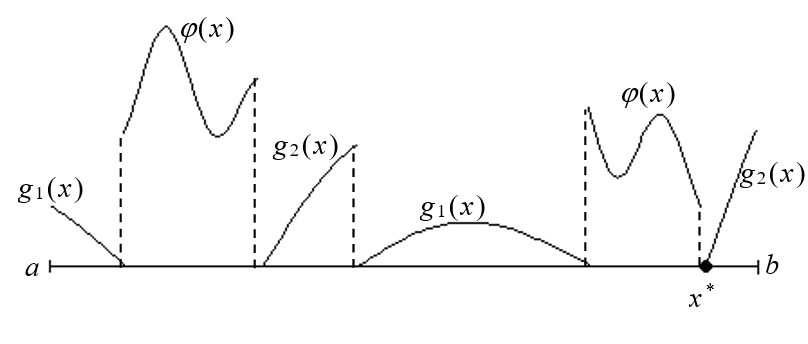
\includegraphics[width=0.8\textwidth]{figures/4_3.png}
  \caption{An ''index'' function}
  \label{fig:4_3}
\end{figure}

Since in the general case the problem \eqref{eq4:problem2} may have no solution (i.e., the feasible subdomain $Q_{m+1}$ might appear to be empty because of the incompatibility of the constrains) an auxiliary problem always having a solution is associated with it. Since conditions \eqref{eq4:condition} are equivalent to the conditions
\begin{displaymath}
  x\in Q_\nu,x\not\in Q_{\nu+1},
\end{displaymath}
this auxiliary problem can be written in the form
\begin{equation}
  \label{eq4:problem3}
  g_M^*=g_M(x_M^*)=\min\{g_M(x):x\in Q_M\},
\end{equation}
where $M$ is the greatest possible value of the index i. e.
\begin{equation}
  1\le M=\max\{\nu(x):x\in[a,b]\}\le m+1
\end{equation}
Since the set $Q_M$ is always nonempty, problem \eqref{eq4:problem3} always has a solution. When $M=m+1$ the solution $x^*=x^*_{m+1}$  is also the solution of the initial problem \eqref{eq4:problem}. When $M<m+1$ the inequality $g_M^*<0$ fulfilled necessarily can be used as an indicator of the incompatibility of the constraints.

The main idea of the index approach is to reduce the constrained problem \eqref{eq4:problem3} to a unconstrained one
\begin{displaymath}
  \psi(x^*)=\min\{\psi(x):x\in[a,b]\},
\end{displaymath}
where
\begin{equation}
  \psi(x)=
  \begin{cases}
    g_\nu(x)/L_\nu, & \nu < M, \\
    (g_M-g_M^*), & \nu=M.
  \end{cases}
\end{equation}

As a result, the arcs of $\psi(x)$ will be Lipschitzian with the constant $L=1$ in each subdomain $Q_\nu,1\le\nu\le M$. A graph of the function $\psi(x)$ for the example (\ref{ex4:problem}) is presented in Fig. \ref{fig:4_4}. This new function will have discontinuities of the first type at the boundary points of the subdomains $Q_\nu$ from \eqref{eq4:q}. Nevertheless, one can estimate the global minimizer $x^*_M$ using the results of $k$ trials for \eqref{eq4:trial} at the points $x_1,\dots, x_k$ in $[a,b]$ (see \cite{strongin1992}).

Indeed, as follows from Lipschitz condition
\begin{equation}
  \label{eq4:lip_opt_est}
  x^*_M\in\{x\in[a,b]:|x-x^i|\ge\psi(x^i),1\le i\le k\}.
\end{equation}

For example, a case for $k=4$ is presented in Fig. \ref{fig:4_4}. The union of the segments highlighted with a bold line in Fig. \ref{fig:4_4} is a complement of the set from the right hand side of \eqref{eq4:lip_opt_est} and does not include the optimum point.
\begin{figure}[ht]
  \centering
  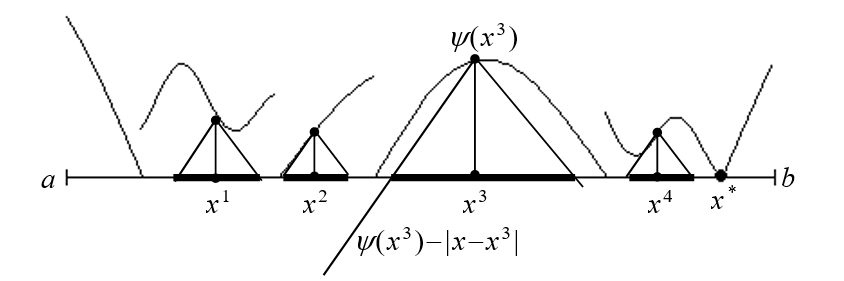
\includegraphics[width=0.8\textwidth]{figures/4_4.png}
  \caption{An estimate of the optimum point}
  \label{fig:4_4}
\end{figure}

Note that the greatest index $M$, the values of Lipschitz constants $L_\nu, 1\le \nu\le M$, and the value of $g_M^*$ are the unknowns. However, these problems can be overcome by means of using instead of them the adaptive estimates of these values obtained in the course of solving the problem on the base of trial results.

Having introduced all necessary concepts, let us turn to the description of the index algorithm.

\section{The index global search algorithm}
The first trial is executed at an arbitrary internal point $x_1\in(a,b)$. The selection of any subsequent trial point $x^{k+1},\; k\ge 1$ is determined by the following rules.

\emph{Rule 1.} Renumber the points $x^1,...,x^k$ of the preceding trials by the lower indices in ascending order of coordinate values, i.e.
\begin{equation}
  \label{eq4:search_data}
  0=x_0<x_1<\dots <x_k<x_{k+1}=1,
\end{equation}
and juxtapose to them the values $z_i=g_\nu(y(x_i)), \; \nu=\nu(x_i), \; 1
\leq i \leq k$, from \eqref{eq4:fx}; the points $x_0=0$ and
$x_{k+1}=1$ are introduced additionally for the convenience  of further notation (the values $z_0$ and $z_{k+1}$ are not defined).

\emph{Rule 2.} Classify the indices $i, \; 1 \leq i \leq k$, of the trial points from set \eqref{eq4:search_data} according to the number of the problem constraints fulfilled at these points, by constructing the sets
\begin{equation}
  I_\nu =\left\{i:1 \leq i \leq k, \; \nu=\nu(x_i) \right\}, \; 1 \leq \nu \leq m+1,
\end{equation}

containing the numbers of all the points $x_i, \; 1 \leq i \leq k$, with
the same values of $\nu$. The end points $x_0=0$ and $x_{k+1}=1$ are
interpreted as the ones having indices equal to zero. An additional set,
$I_0=\left\{0,k+1\right\}$, corresponds to them.

\emph{Rule 3.} Determine the maximum value of the index:
\begin{equation}
  M=\max\left\{\nu(x_i), \; 1 \leq i \leq k \right \}.
\end{equation}

\emph{Rule 4.} Compute the current lower estimates,
\begin{equation}
  \label{eq4:lip_est}
  \mu = \max\left\{ \frac{\left|z_i-z_j\right|}{ x_i - x_j }, \; i,j \in I_\nu, \; i>j \right\},
\end{equation}
for the unknown Lipschitz constants $L_\nu$ of the functions $g_\nu(y),1
\leq \nu \leq m+1$. If a set $I_\nu$ contains less than two elements, or
if $\mu_\nu$ is equal to zero, then assume $\mu_\nu=1$. As follows from \eqref{eq4:lip_est}, the estimates $\mu_\nu$ are non-decreasing starting from the moment when \eqref{eq4:lip_est} generates a positive value $\mu_\nu$.

\emph{Rule 5.} For all nonempty sets $I_\nu, \; 1 \leq \nu \leq m+1$, compute the estimates
\begin{equation}
  \label{eq4:z_const}
  z_\nu^\ast = \left\{
  \begin{array}{lr}
    0, & \nu < M,\\
    \min\{ g_\nu(y(x_i): i\in I_\nu \}, & \nu = M.
  \end{array}
  \right.
\end{equation}

\emph{Rule 6.} For each interval ($x_{i-1},x_i), \; 1 \leq i \leq k+1,$ compute the \textit{characteristics} $R(i)$:
\begin{gather}
  \label{eq4:characteristic}
  R(i)=2\Delta_i-4\frac{z_i-z_\nu^\ast}{r_\nu \mu_\nu}, \; \nu=\nu(x_i)>\nu(x_{i-1}), \nonumber \\
  R(i)=\Delta_i+\frac{(z_i-z_{i-1})^2}{r_\nu^2 \mu_\nu^2\Delta_i}-2\frac{z_i+z_{i-1}-2z_\nu^\ast}{r_\nu \mu_\nu}, \;  \nu=\nu(x_i)=\nu(x_{i-1}),\\
  R(i)=2\Delta_i-4\frac{z_{i-1}-z_\nu^\ast}{r_\nu \mu_\nu}, \; \nu=\nu(x_{i-1})>\nu(x_i), \nonumber \\
  \Delta_i=x_i - x_{i-1} \nonumber
\end{gather}
The values $r_\nu>1, 1\le\nu\le m+1$ are the parameters of the algorithm. An appropriate choice of the values $r_\nu$ allows using the products $r_\nu\mu_\nu$ as the estimates of Lipschitz constants $L_\nu, 1\le\nu\le m+1$.

\emph{Rule 7.} Find the interval $(x_{t-1},x_t)$ with the maximum characteristic
\begin{equation}
\label{eq4:MaxR}
R(t)=\max{\left\{R(i): 1 \leq i \leq k+1\right\}}.
\end{equation}

\emph{Rule 8.} Make the next trial at the midpoint of the interval
$(x_{t-1},x_t)$ if the indices of the points $x_{t-1}$ and $x_t$  are not the same, i.e.
\[
x^{k+1} = \frac{x_t + x_{t-1}}{2}, \; \nu(x_{t-1}) \neq \nu(x_t).
\]
Otherwise, make the trial at the point
\begin{equation}
\label{eq4:next_point}
x^{k+1} = \frac{x_t+x_{t-1}}{2} - \frac{z_t-z_{t-1}}{2r_\nu\mu_\nu},\; \nu=\nu(x_{t-1})=\nu(x_t).
\end{equation}

The described rules can be supplemented with the termination condition, finalizing the iterations of the method if
\begin{equation}
\label{eq4:stop_cond}
  x_t - x_{t-1}\le\epsilon
\end{equation}
where $t$ from \eqref{eq4:MaxR} and $\epsilon>0$ is the predefined accuracy of the optimization.

Let us formulate the conditions of convergence for the algorithm in the form of the following theorem.
\begin{theorem}
Let the considered index algorithm be applied to the solving of problem \eqref{eq4:problem} and the following conditions be satisfied:
\begin{enumerate}
  \item each function $gj, 1\le j\le m+1$ satisfies Lipschitz condition with the constant $L_j$ in the interval $[a,b]$, i.e.,
  \[
  |g_j(x_1)-g_j(x_2)|\le L_j|x_1-x_2|,\; 1\le j\le m+1,\; x_1,x_2 \in[a,b]
  \]
  \item the following inequalities hold for the quantities $\mu_\nu$ from \eqref{eq4:lip_est} starting from some step
  \[
  r_\nu\mu_\nu > 2L_\nu,\; 1\le\nu \leq m+1.
  \]
\end{enumerate}

Then the set of the limit points of the sequence $\{x_k\}$ generated by the index algorithm coincides with the set of solutions of problem \eqref{eq4:problem} with $\epsilon=0$ and termination criterion \eqref{eq4:stop_cond}. In addition, the index of each limit point equals to $M$ and the convergence to any limit point $\overline{x}$  is bilateral if $\overline{x}\not=a$ and $\overline{x}\not=b$.
\end{theorem}

This theorem is given without a proof, which can be found, for example, in \cite{stronginMarkin1986, stronginMarkin1987}. Various modifications of this algorithm and the corresponding theory of convergence are given in \cite{SergeyevFamularoPugliese2001,barkalovStrongin2002,SergeyevFamularoPugliese2003,sergeyev2006,sergeyevKhalafKvasov2007,sergeyevKvasovKhalaf2007}.

\textbf{The results of the experiment.} Let us consider a problem from Example (\ref{ex4:problem}) as an illustration. Under assumption of partial computability the arcs of the problem functions corresponding to the domains $Q_j, 1\le j\le 3$, from \eqref{eq4:q} are presented in Fig. \ref{fig:4_6}.

Three methods have been used for solving this example:
\begin{enumerate}

  \item Scanning a uniform grid with the precision (distance between adjacent nodes) $\epsilon=10^{-5}$.
  \item Penalty function method, i.e., the minimization of the function
  \[
  p(x)=\varphi(x)+(\max\{g_1(x),0\})^2+(\max\{g_2(x),0\})^2
  \]
  using Algorithm of Global Search. The coordinates of the trial points executed by AGS in the process of problem solving are marked by the vertical strokes in Fig. \ref{fig:4_5}. The coordinates of the trials executed in the close points are marked by a dark rectangle.
  \item Index algorithm with the parameters $r_\nu=2, 1\le \nu \le 3$, and $\epsilon =10^{- 5}$. The trial point coordinates executed by the algorithm in the course of problem solving are marked by three rows of the vertical strokes in Fig. \ref{fig:4_6}. The strokes in the upper row correspond to the points with the index $\nu=1$, the ones of the second row --- to the points, the indices of which are equal to 2; and the points marked by the strokes in the bottom row are the feasible ones. The trial coordinates performed in the close points are marked by a dark rectangle.
\end{enumerate}

\begin{figure}[ht]
  \centering
  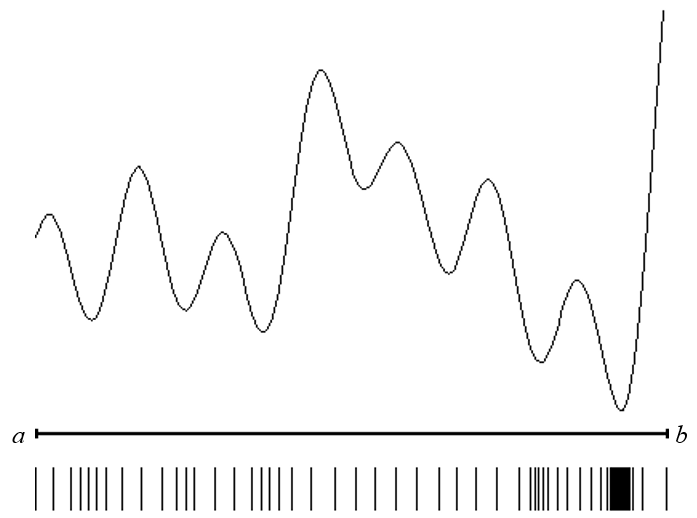
\includegraphics[width=0.8\textwidth]{figures/4_5.png}
  \caption{Minimization by means of Penalty Function Method}
  \label{fig:4_5}
\end{figure}

It is worth noting, that in the applied problems the estimates of the constraints as well as of the objective functions require considerable computation resources very often. The results presented in Table \ref{tab4:exp_results} confirm the effectiveness of the index scheme of the account of
constraints.

\begin{table}
  \caption{The results of solving the test problem}
\begin{center}
  \label{tab4:exp_results}
  \begin{tabular}{cccc}
    \hline
    Method & $k_1$ & $k_2$ & $k_3$ \\ \hline
    Uniform grid technique  & 160000 & 90280 & 56476 \\ 
    Penalty Function Method &  375 & 375 & 375 \\ 
    Index method & 63 & 49 & 35 \\ \hline
  \end{tabular}
\end{center}
\end{table}

Here $k_i$ is the number of computations of the $i$ problem function, i.e., of the function $g_i(x )$.
\begin{figure}[ht]
  \centering
  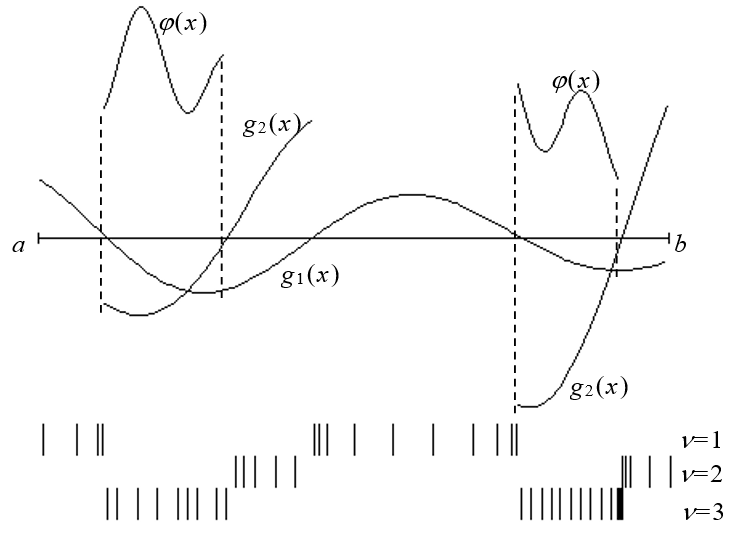
\includegraphics[width=0.8\textwidth]{figures/4_6.png}
  \caption{The minimization of an ``index'' function}
  \label{fig:4_6}
\end{figure}

\section{Index algorithm taking into account the existence of $\epsilon$-reserved solutions}
Let us return to the consideration of a one-dimensional problem of the kind \eqref{eq4:problem}
\begin{displaymath}
  \varphi(x^*)=\min\{\varphi(x):x\in [a,b],\; g_j(x)\le 0, \; 1\le j\le m\}
\end{displaymath}
In the case when the objective function and the left-side parts of the constraints are partially computable, it is necessary to use the form \eqref{eq4:problem2}.
\example
{
Let us consider problem \eqref{eq4:problem} with $x\in[0.6,2.2]$, $m=3$ as an illustration:
\begin{gather*}
\varphi(x)=\cos(18x-3)\sin(10x-7)+1, \\
g_1(x)=\exp(-x/2)\sin(6x-1.5) \\
g_2(x)=\sin(4x-2.2)+\cos(6x-2.9) \\
g_3(x)=|x|\sin(2\pi x - 0.5).
\end{gather*}
}
\begin{figure}[ht]
  \centering
  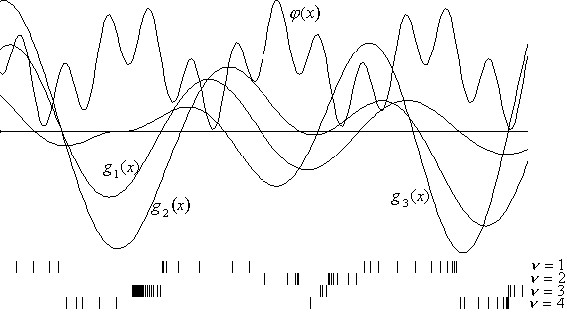
\includegraphics[width=0.8\textwidth]{figures/4_7.jpg}
  \caption{The solution of a problem by Index Method}
  \label{fig:4_7}
\end{figure}
The functions $g_j , 1\le j\le 4$, are pictured in Fig. \ref{fig:4_7}. Assuming a partial calculability, the arcs of
the functions corresponding to the domains $Q_j ,1\le j\le 4$, from \eqref{eq4:q} are presented in Fig. \ref{fig:4_8}.

\begin{figure}[ht]
  \centering
  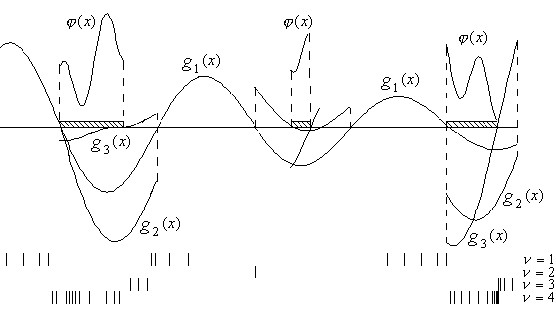
\includegraphics[width=0.8\textwidth]{figures/4_8.jpg}
  \caption{The problem solving by Index Method with the $\epsilon$-reservs}
  \label{fig:4_8}
\end{figure}

Index algorithm described in Sec. 3.3 was used to solve this example with $x_1=(a+b)/2$, $r=2$, and $\varepsilon=10^{-5}$. The coordinates of 102 trial points executed by the algorithm in the process of problem solving are marked by four rows of the vertical strokes in Fig. \ref{fig:4_7}. The strokes of the upper row correspond to the points with the index $\nu=1$, the ones of the second and the third rows --- to the points, the indices of which are equal to 2 and 3, respectively; and the points
marked by the strokes of the bottom row are feasible.

The coordinates of the trials executed in the close points are marked by a dark rectangle. The values of the functions $g_1 , g_2 , g_3$ , and $\varphi=g_4$ have been computed $k_1=102$, $k_2=80, k_3=64,$ and $k_4=26$ times, respectively. As one can see in Fig. \ref{fig:4_7}, the trial points concentration takes place not only in the vicinity of the point of the global optimum $x^*=2,07957$, but also in the vicinities of the inadmissible boundary points of the domains $Q_j$ from \eqref{eq4:q}. This effect can be reduced by the substitution of estimates \eqref{eq4:z_const} by the estimates
\begin{equation}
  z_\nu^\ast = \left\{
  \begin{array}{lr}
    -\epsilon_\nu, & \nu < M,\\
    \min\{ g_\nu(y(x_i): i\in I_\nu \}, & \nu = M.
  \end{array}
  \right.
\end{equation}
where $\epsilon_R=(\epsilon_1 ,\dots, \epsilon_m)$ is a predefined vector with positive components. Thus, $z^*=0$ if there exist the points $x_i,1\le i\le k$ from series \eqref{eq4:search_data} with the index greater than $\nu$. As a consequence of this substitution the values of the characteristics $R(i)$ from \eqref{eq4:characteristic} will become lower (because of the subtraction of $\epsilon_\nu$) if
\begin{equation}
  \nu=\max\{\nu(x_{i-1},\nu(x_i)\}<\max\{\nu(x_j):1\le j\le k\}\le V
\end{equation}
that makes executing the trials in the corresponding intervals  ($x_{i-1}$ , $x_i$ ) less probable. In all other aspects, the algorithm remains the same.

This \emph{prima facie} mechanical trick has a well-established theoretical basis considered below.

\begin{definition}
  The point $x_\epsilon$ is called an $\epsilon$-reserved solution of problem \eqref{eq4:problem} if the condition
  \begin{equation}
    \label{eq4:eps_res_problem}
    \varphi(x_\epsilon)=\min\{\varphi(x):x\in [a,b], g_j(x)\le -\epsilon_j,1\le j\le m\}
  \end{equation}
  meets where $\epsilon_1, \dots,\epsilon_m$ are the positive values of reserve for each constraint. Let us introduce into consideration also the set
  \begin{equation}
    \label{eq4:x_epsilon}
    X_\epsilon = \{x\in[a,b]:g_j(x)\le 0, 1\le j\le m, \varphi(x)\le\varphi(x_\epsilon)\}
  \end{equation}
  of all feasible solutions of the problem, which are no worse with respect to the objective function value than the $\epsilon$-reserved solution.
\end{definition}

The existence of the $\epsilon$-reserved solution of problem \eqref{eq4:problem} can be interpreted as some analogue of the conditions of regularity in the classical nonlinear programming problems. The applied role of this condition should be noted also. Even if the exact solution $x^*$ is known, its practical implementation is possible as some approximation to $x^*$ only. Therefore, the existence of the feasible points from $Q$ close to $x^*$ (with respect to the coordinates and to the objective
function values) is important. The existence of the $\epsilon$-reserved solution guarantees the availability of such points. Moreover, the domain $X_\epsilon$ may play a role of the set of suitable approximations.

The index algorithm with the $\epsilon$-reserves has been applied to the considered example with $\epsilon_i=0.2, 1\le i\le 3$. The search trial coordinates are marked by the vertical strokes in Fig. \ref{fig:4_8}. The solution has required 52 trials only and provided the same precision of the problem solution as in
the case when the vector $\epsilon_R$ equals to zero. Moreover, the values of the functions $g_1$ , $g_2$ , $g 3$ , and $\varphi=g_4$ have been calculated $k_1 =52$, $k_2 =39$, $k_3 =38$, and $k_4 =25$ times, respectively.

The conditions of convergence for the algorithm are presented in the following theorem (given without proof, see \cite{}).

\begin{theorem}
  Assume problem \eqref{eq4:problem} to have a solution $x^*$ and the following conditions to be satisfied:
  \begin{enumerate}
    \item each domain $Q_j ,1\le j\le m+1$ from \eqref{eq4:q} is a union of a finite number of positive length segments;
    \item each function $g_j ,1\le j\le m+1$ allows Lipschitz extension $G_j (x)$ with the constant $L_j$ over the whole interval $[a,b]$, i.e.,
    \begin{equation}
      g_j(x)=G_j(x),x\in Q_j,1\le j\le m+1;
    \end{equation}
    \item the components $\epsilon_\nu$ of the reserve vector $\epsilon_R$ corresponding to the constraints being active at the absolute minimum point $x^*$ (i.e., the constraints, for which $g_\nu(x^*)=0$) satisfy the inequalities
    \begin{equation}
      \label{eq4:reserves}
      0<2\epsilon_\nu<L_\nu(\beta-\alpha)
    \end{equation}
    where $\beta-\alpha$ is the length of the interval $[\alpha,\beta]\subset Q_{m + 1}$ containing the point $x^*$;
    \item the components $\epsilon_\nu$ of the reserve vector $\epsilon_R$ corresponding to the constraints which are not active at the absolute minimum point $x^*$ (i.e., $g_\nu(x^* )<0)$ satisfy either inequalities \eqref{eq4:reserves} or the inequalities
    \begin{equation}
      0< \epsilon_\nu <|g_\nu (x^* )|;
    \end{equation}
  \end{enumerate}

  Then:
  \begin{enumerate}
    \item the point $x^*$ is the limit point of the trial sequence $\{x_k \}$ generated by index algorithm for problem \eqref{eq4:problem} at $\epsilon =0$ in the termination condition \eqref{eq4:stop_cond};
    \item any limit point $\overline x$ of the sequence ${x_k }$ is a solution of the problem \eqref{eq4:problem};
    \item the convergence to the limit point $x$ is a bilateral one if $x\not=a$ and $x\not=b$.
    If the conditions \eqref{eq4:reserves} and (4.27) are not satisfied for given vector of reserves $\epsilon_R$ but the
    problem $\eqref{eq4:problem}$ has an $\epsilon$-reserved solution $x_\epsilon$ defined by \eqref{eq4:eps_res_problem}, then:

    \item for any limit point $x$ of the sequence ${x_k}$ it is true that
    \begin{displaymath}
      \varphi(\overline x)=\inf\{\varphi(x^k):g_j(x^k)\le 0,\: 1\le j\le m,\: k=1,2,\dots\}\le\varphi(x_\epsilon);
    \end{displaymath}
    \item any limit point $\overline x$ is a boundary point of the set $X_\epsilon$ from \eqref{eq4:x_epsilon} if the function $\varphi(x)$ has no more than one point of local maximum in each of the isolated intervals making up the set $X_\epsilon$;
    \item the above statement on the bilateral character of the convergence remains in force.
  \end{enumerate}
\end{theorem}

As it has been demonstrated by the experiment with solving the example described above, the increase of the reserve values may result in an essential decrease of the trial concentration in the boundary points of non-feasible domains. The theoretical properties of the trial sequences generated by the index algorithm are determined by the following statement (see the proof in \cite{stronginSergeyev2000} also).
\begin{theorem}
  Assume the convergence conditions for the index algorithm to be satisfied and the inequalities
  \begin{displaymath}
    g_\nu(x)\ge\delta_\nu,x\in[\alpha,\beta],\delta_\nu\ge 0
  \end{displaymath}
  to be satisfied in a subinterval $[\alpha,\beta]\subset Q_\nu \: 1\le\nu\le m$, the length of which meets the condition
  \begin{displaymath}
    \beta-\alpha>\frac{2(r_\nu-1)(\delta_\nu+\epsilon_\nu)}{r^2_\nu L_\nu}.
  \end{displaymath}

  Then for the density $P_{\alpha\beta}$ of the points from the sequence $\{x_k\}$ generated by the index algorithm while solving the problem \eqref{eq4:problem} there is the estimate
  \begin{displaymath}
    P_{\alpha\beta}<\frac{r^2_\nu L_\nu}{(r_\nu-1)(\delta_\nu+\epsilon_\nu)}.
  \end{displaymath}
\end{theorem}

\textbf{Selection of components of the vector of reserves.} A problem of the choice of concrete component values in the vector of reserves $\epsilon_R$ arises when applying the considered algorithm.
The convergence theorem can help in solving this problem. Condition \eqref{eq4:reserves} can be considered as a recommendation for the selection of the reserve values, for which the property of
convergence to the solution of problem \eqref{ex4:problem} remains. However, in the general case the values of Lipschitz constants are not given \emph{a priori}, and the length of the interval $[\alpha,\beta]$ from $Q_{m + 1}$, including the sought solution $x^*$ is not kwon also. These difficulties are possible to avoid by
substitution of the unknown coefficients $L_j,\: 1\le j\le m$, by their adaptive underestimates $\mu_\nu$ from (4.15) and by assumption that $\beta-\alpha>\delta=\epsilon q$ where $\epsilon >0$ (accuracy) is a parameter defined in the termination condition and the factor $q>1$ can be interpreted as an a priori estimate of how many times the length of the interval $[\alpha,\beta]$ is greater than given accuracy $\epsilon$. As a result, one can take
the reserve estimates in the form (adaptive reserves)
\begin{displaymath}
  \epsilon_\nu=\mu_\nu\delta,\: 1\le\nu\le m.
\end{displaymath}

\textbf{The results of the experiment.} In order to demonstrate the efficiency of the adaptive reserves, a series of problems with the multiextremal constraints has been solved.

Let us consider a generator $G$ generating the problems with $m$ constraints on the base of a random mechanism $F$ producing the functions $f(x),\: x \in [ a , b ]$. The rules determining the
functioning of this mechanism $G$ consist in the following.
\begin{enumerate}
  \item $m+1$ functions $f_j(x),\: 1\le j \le m+1,\: x\in[a,b]$, are generated independently by means of given mechanism $F$.
  \item The minimax value
  \begin{displaymath}
    \Delta=\min_{a\le x\le b}\max_{1\le j\le m}f_j(x),
  \end{displaymath}
  is calculated and the left-hand parts of the constraints
  \begin{equation}
    \label{eq4:generated_g}
    g_j(x)=f_j(x)-\Delta\delta,\: 1\le i\le m,
  \end{equation}
  which a nonempty feasible domain $Q$ corresponds to at $\delta>0$ are introduced. Increasing the value of the parameter $\delta$ allows to expand the feasible domain.
  \item Function \eqref{eq4:generated_g} and the objective function $\varphi(x)=f_{m+1}( x )$ form a problem of the kind \eqref{eq4:problem} obviously having a solution.
\end{enumerate}

In the cases, when it is necessary to denote the parameters $m$ and $\delta$ used by the generator during its functioning, let us use the notation $G ( m , \delta )$. In the experiments, the results of whichare presented below two generators were employed. One of these (let us denote it as $G_{SH} ( 5 , 1 ) )$ was based on the function
\begin{displaymath}
  \varphi(x)=-\sum_{j=1}^{10}\frac{1}{(K_j(x-A_j)^2+C_j)},\; x\in[0,10].
\end{displaymath}
$1\le K_j\le 3,\: 0\le A_j,\: C_j\le 10 $, where the parameters $K_j,\: A_j,\: C_j ,\: 1 \le j \le 10$ are the independent random variables distributed uniformly over the intervals specified above. The second generator hereinafter denoted as $G_{HL} ( 5 , 1 ) )$ was based on the function
\begin{equation}
  \varphi(x)=\sum_{j=1}^{14}(A_j\sin(2j\pi x) + B_j\cos(2j\pi x)),\: x\in[0,1]
\end{equation}
where the values of the parameters $A_j,\: B_j,\: 1 \le j \le 14$, are distributed independently and uniformly over the interval $[-1 ,1 ]$. Both generators were applied to the generation of 100 own
problems of the kind \eqref{eq4:problem}.

The problems were solved by the initial index algorithm as well as by the algorithm with $\epsilon$-reservation. The parameters $r_\nu ,\: 1 \le \nu \le 6$, from (4.17) were chosen as
\begin{displaymath}
  r_\nu = \left\{
  \begin{array}{lr}
    \gamma, & k_\nu < 20\\
    2, & k_\nu \ge 20
  \end{array}
  \right.,
\end{displaymath}
where $k_\nu$ is the number of the computed values of the function $g_\nu$ (i.e., the cardinality of the set $I_\nu$). In the test set generated by generator $G_{SH}$ the values $\gamma=20,\: \epsilon = 0.001$ and the reserves $\delta_\nu=0.02,\: 1 \le \nu \le 5$, were used in the experiments. For the problems from the second test set
(generated by $G_{HL}$ ) the values $\gamma = 10, \epsilon=0.0001$ and the parameters $\delta_\nu=0.001,\: 1 \le \nu\le 5$, were used.

\begin{figure}[ht]
  \centering
  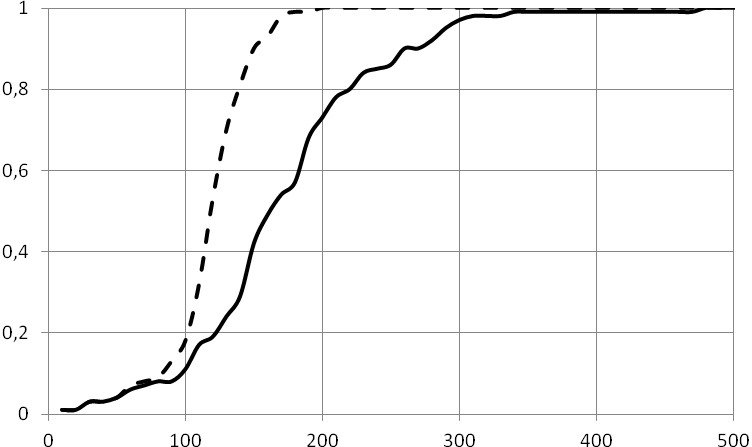
\includegraphics[width=0.8\textwidth]{figures/4_9.png}
  \caption{The operation characteristics in class $G_{SH}$}
  \label{fig:4_9}
\end{figure}

\begin{figure}[ht]
  \centering
  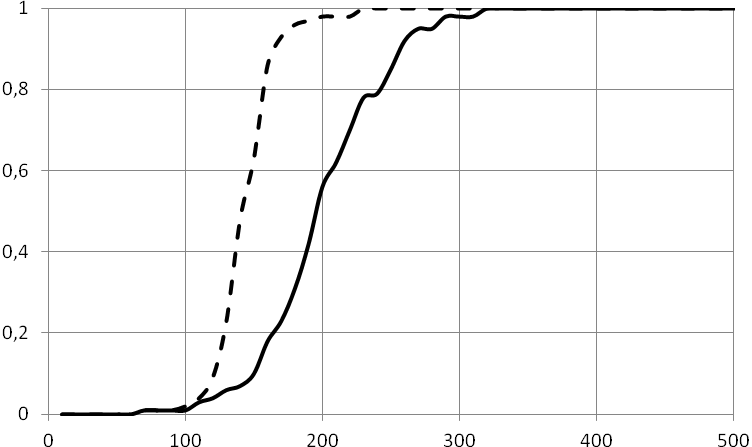
\includegraphics[width=0.8\textwidth]{figures/4_10.png}
  \caption{The operation characteristics in class $G_{HL}$}
  \label{fig:4_10}
\end{figure}

The operational characteristics for both method obtained for the test problem sets generated by $G_{SH}$ and $G_{HL}$ are presented in Figures \ref{fig:4_9} and \ref{fig:4_10}, respectively. The lower (solid) curves refer to the initial index algorithm while the upper (dashed) ones correspond to the index algorithm with the adaptive reserves. Such arrangement of the curves demonstrates the algorithm with the
adaptive reserves to provide much faster obtaining the estimates falling into given vicinity of the solution than the initial index algorithm. The average numbers of iterations for the method
without the reserves and for the method with the adaptive reserves were equal to 171 and 117 for the problems $G_{SH}$ and 199 and 142 for the ones $G_{HL}$ , respectively.

\section{Index method with adaptive order of checking for constraints}
According to the rules of the index method considered in the preceding subsections, every trial includes the successive check of the fulfilment of the problem constraints in the corresponding point of the search domain. The finding of the first violated constraint terminates the trial and initiates the transition to the next iteration. If a numeration of the constraints in the increasing order by the computational costs of their checking is introduced (i.e., if the simpler constraints are checked first) one can reduce essentially the overall computational costs in the course of optimization. The above is important for the problems, in which the estimating of the function value requires a considerable computational resources connected with a necessity of the numerical modelling of the behavior of the systems described by these functions (as it takes place, for example, in numerous problems of the optimal design).

Obviously, the computational expenditures of the trial execution depend on the order of the problem functions’ computation essentially. If the calculation time of any problem is independent on the iteration execution point, the less the number of the problem functions (constraints and objective function) calculated at a point x, the less the trial execution costs in this point.

For many applied problems, it is naturally to assume that a constraint violated at a point in the search domain, will be violated in some neighbourhood of this point as well. In this case, it might be useful to begin the next trials in the points of this neighbourhood with checking the fulfilment of this particular constraint. In the scope of the above, it seems reasonable to design a global optimization algorithm allowing the modification of the constraint  check order taking into account the information obtained during the search. The check order design will be oriented onto the constraint violated at an iteration point to be found as early as possible.

Let us now turn to the generalization of the scheme described in sections 3.3 and 3.4 onto the case when the constraint check order is not a fixed one. For further consideration, the initial algorithm described above will be referred to as \emph{Fixed Check Order Method} (FCOM).

The algorithm proposed below allows the modification of the constraint order check during solving the problem \eqref{eq4:problem}. These modifications are firstly directed onto analyzing during the current iteration the constraint violated at the end of the interval including the current iteration point. As it has been already mentioned above, such an approach might reduce the number of checks at the new trial point since the violation of this constraint in a vicinity of already found violation might be quite probable. Hence, the need in new rules for the juxtaposition of the indices to the points from \eqref{eq4:search_data} (remind, that these indices determine the use of expressions \eqref{eq4:characteristic} for the computation of the characteristics) as well as in a special order
of the constraint check at the current trial point arises. Note that the formation of such order is inessential for the intervals, the ends of which belong to a feasible domain $Q$ from \eqref{eq4:Q_union} since a necessity for checking all constraints is probable in such intervals.

Assume the constraint with the number $j,\: 1\le j\le m$, is fulfilled at all points of the domain
\begin{equation}
  Q_j=\{x\in[a,b]:g_j(x)\le 0\},\: 1\le j\le m,
\end{equation}
which hereinafter will be called the feasible domain for this constraint. The feasible domain $Q$ of initial problem \eqref{eq4:problem} can be defined by the condition
\begin{equation}
  \label{eq4:Q_union}
  Q=Q_1\cap\dots\cap Q_m.
\end{equation}

\textbf{The constraints’ check order.} he numbering of the constraints and the objective function introduced in the statement of problem \eqref{eq4:problem} and defined by the sequence of integer numbers
\begin{equation}
  \label{eq4:basic_h}
  H=\{1,2,\dots,m,m+1\},
\end{equation}
will be considered as a base one.
Assume that every particular point $x$ from the search domain $[a,b]$ can have its own order of the problem constraints’ checking. The order of such checking corresponding to the point $x_i$ from (4.12) will be defines as some permutation $H(x_i )$ of the basic numbers from \eqref{eq4:basic_h}, i.e.,
\begin{equation}
  H(x_i)=\{j_{i1},\dots,j_{im},j_{i,m+1}\},\:0\le i\le k,
\end{equation}
where
\begin{equation}
  j_{i,m+1}=m+1,\:0\le i\le k.
\end{equation}

Since the constraints’ check order while the trial execution at the point $x$ i is determined by the corresponding tuple $H(x_i )$ from (4.33), the termination of the trial at this point after the computation of the values of l problem functions produces the value $z_i=g_\nu(x_i)$ where $\nu=j_{il}$. In this connection, let us use not the serial number $l$ of the last function calculated in this point, as it was accepted in (4.7) but the index of the last function in the basic numeration (4.32) as the
value of $\nu(x_i )$ for the point $x_i$ , i.e.,
\begin{equation}
  \nu(x_i)=j_{il}.
\end{equation}

\textbf{Algorithm.} The trial selection rules for Fixed Check Order Method (FCOM) already considered above give the base of the new algorithm scheme, which will be called \emph{Adaptive
Check Order Method} (ACOM). Since the alterable constraint check order excludes a possibility to use expression (4.13) to determine the sets $I\nu$, to construct them, an information array connecting each $x_i$ from (4.12) with the indices of all functions, which have been computed in this node is necessary. Hereinafter, the existence of such database is presumed. The rest modifications consist in the following.

\emph{Modification 1 (the fixation of the check order)}. Each point $x_i$ from \eqref{eq4:search_data} is assigned the corresponding checking order $H(x_i )$ from (4.33), and this order is included into the algorithm database.

\emph{Modification 2 (the determination of the trial points’ indices).} Each point $x_i$ from \eqref{eq4:search_data} is assigned the value $z_i=g_\nu(x_i)$ where according to (4.35), the index $\nu=\nu(x_i)$ is the basic index from (4.32) corresponding to the value of the last function estimated in this point. These indices are used in all computations based on expressions (4.13)– (4.17), (4.19).

The modifications in the method of using the indices are related to rules (4.17) of calculations of the characteristics $R(i)$ of the intervals $(x_{i-1},x_i),\: 1\le i\le k$, with noncoincident
indices of the boundary points only. Assume
\begin{equation}
  \nu(x_{i-1})=j_{i-1,p}=j_{i,q}\not=\nu(x_i)=j_{i-1,u}=j_{i,x},
\end{equation}
i.e., the problem function with the basic index $\nu(x_{i-1})$ has the index $p$ in the sequence $H(x_{i-1})$ corresponding to the point $x_{i-1}$ and the index $q$ in the sequence $H(x_i)$ corresponding to the point $x_i$. Analogously, the function with the basic index $\nu(x_i)$ corresponds to the index $u$ from the sequence $H(x_{i-1})$ and the index s from the sequence $H(x_i)$. Then, the introduced modification altering the sixth rule of FCOM consists in the following.

If for the indices $p,q, u$ and $s$ from (4.36) the conditions
\begin{equation}
  p<u,q<s,
\end{equation}
are fulfilled, in order to determine the characteristic $R(i)$ one should use the second expression from formulae (4.17) with $\nu=\nu(x_i)$ (note that in this case the value $g_\nu(x_{i-1})$ is undefined).

Otherwise, when the reverse to (4.37) conditions are fulfilled
\begin{equation}
  p>u,q>s,
\end{equation}
the characteristic $R(i)$ is defined by the third expression from (4.17) with $\nu=\nu(x_{i-1})$ (in this
case, the value $g_\nu(x_i ) is undefined)$. In the cases when conditions (4.37) and (4.38) are not fulfilled, the initial order of calculations prescribed by the sixth rule of the initial algorithm remains.

\emph{Modification 3 (the choice of the constraints’ check order in the current trial point).} Assume that the constraints’ check order corresponding to the first two trial points is defined by
the conditions
\begin{equation}
  H(a)=H(b)=H,
\end{equation}
where $H$ from (4.32). Let
\begin{displaymath}
  p=\nu(x_{t-1}),\: q=\nu(x_t)
\end{displaymath}
are the indices of the boundary points of the interval $(x_{t-1},x_t)$ including the current trial point $x^{k+1}$ (according to the eighth rule) determined according to (4.35). Let us introduce a notation $\{s,H\backslash s\}$ for the tuple obtained from $H$ by excluding the index $s$, shifting all indices $1,2,\dots,s-1$ to the right of one position, and the transfer of the index s excluded from $H$ into the first position, i.e.,
\begin{displaymath}
  \{s,H\backslash s\}=\{s,1,2,\dots,s-1,s+1,\dots,q-1,q+1,\dots,m+1\}.
\end{displaymath}
When $1\le p\le q\le m$, the superposition of the operations of the type described above produces the tuple of the kind
\begin{displaymath}
  \{p,\{q,H\backslash q\}\backslash p\}=\{p,q,1,\dots,p-1,p+1,\dots,q-1,q+1,\dots,m+1\}.
\end{displaymath}
Note that according to (4.34), the index $m+1$ always occupies the last position.

Now let us agree to determine the order $H(x^{k+1}),\: k\ge 1$ according to the following rules:
\begin{gather}
 H(x^{k+1})=H,\: p=q=m+1, \nonumber \\
 H(x^{k+1})=\{p,H\backslash p\}, (p=q<m+1)\cup(p<q=m+1), \nonumber \\
 H(x^{k+1})=\{q,H\backslash q\}, p=m+1>q\\
 H(x^{k+1})=\{p, \{q,H\backslash q\}\backslash p\}, p<q\le m \nonumber \\
 H(x^{k+1})=\{q, \{p,H\backslash p\}\backslash q\} m\ge p>q. \nonumber
\end{gather}

\textbf{Note.} While solving the problem \eqref{eq4:problem} rules (4.39) and (4.40) included into the scheme of ACOM assign the index values from (4.35) to all trial points unambiguously. Then, any feasible point $x$ always corresponds to the index $\nu(x)=m+1$. This value can be predicted before the trial execution in such point as well. However, if the point $x$ is not a feasible one and does not belong to the points, in which the trials have been executed already, the index value can be undefined in this point.

The convergence conditions for the algorithm are formulated in the following theorem.

\begin{theorem}
Assume problem \eqref{eq4:problem} to have a solution $x^*$ and the following conditions are fulfilled:
\begin{enumerate}
  \item each domain $Q_j ,1\le j\le m+1$ from (4.30) represents a union of a finite number of segments with a positive length;
  \item each function $g_j(x): 1\le j\le m+1$ satisfies Lipschitz condition with the corresponding constant $L_j$;
  \item the components $\epsilon_\nu$ of the reserve vector $\epsilon_R$ satisfy the inequalities
  \begin{equation}
    0<2\epsilon_\nu<L_\nu(\beta-\alpha),
  \end{equation}
  where $\beta-\alpha$ is the length of the interval $[\alpha,\beta]$ belonging to the feasible domain $Q$ from \eqref{eq4:Q_union} and including the point $x^*$, which is the solution of the problem;
  \item since some sufficiently large step number $k$ the values $\mu_\nu$ from (4.15) corresponding to the nonempty sets $I_\nu$ satisfy the inequalities
  \begin{displaymath}
    r_\nu\mu_\nu>2L_\nu,\: 1\le\nu\le m+1,
  \end{displaymath}
  where $r_\nu>1,\: 1\le\nu\le m+1$ are the parameters of the algorithm.
\end{enumerate}

  Then:
  \begin{enumerate}
    \item the point $x^*$ is a limit point of the sequence $\{x_k\}$ generated by the described method with the adaptive constraint check order for problem \eqref{eq4:problem} at $\epsilon=0$ in termination condition \eqref{eq4:stop_cond};
    \item any limit point $x$ of the sequence $\{x_k\}$ is a solution of problem \eqref{eq4:problem};
    \item the convergence to the limit point $\overline x$ is bilateral if $\overline x\not= a$ and $\overline x\not=b$.
  \end{enumerate}
\end{theorem}

\textbf{Proof} of the theorem is given in \cite{SergeyevFamularoPugliese2001}.

\textbf{The results of the experiments.} Let us consider solving of the problem from Example \ref{ex4:problem} using ACOM with the parameters $r_\nu=2, \epsilon_\nu=0,\: 1\le \nu\le 3$, and $\epsilon=10^{-5}$ in the termination criterion as an illustration. The trial point coordinates executed by the algorithm during the
problem solving practically coincide to the ones marked by three rows of the vertical strokes in Fig. 4.6. However, the number of the computations of the constraint values appears to be different for FCOM and ACOM. In the fixed constraints’ check order the function values have been calculated $k_1 =63,\: k_2 =49,\: k_3 =35$ times while in the adaptive order --- $k_1 =52,\: k_2 =48,\:
k_3 =35$ times. These results are evidence of the decrease of the number of such checks when using ACOM even for the example with two constraints. The efficiency of the proposed scheme reveals itself more clearly when solving the problems with many constraints.

With this purpose, let us return to solving the problem series produced by generators $G_{SH}(5,1)$ and $G_{HL} (5,1)$ described in section 3.4. Both generators were applied to the generation of
its own set of 1000 problems of the kind \eqref{eq4:problem}.

\begin{figure}[ht]
  \centering
  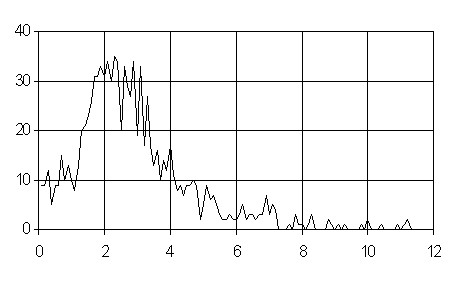
\includegraphics[width=0.8\textwidth]{figures/4_11.jpg}
  \caption{The distribution of problems of the class $G_{SH}$}
  \label{fig:4_11}
\end{figure}

\begin{figure}[ht]
  \centering
  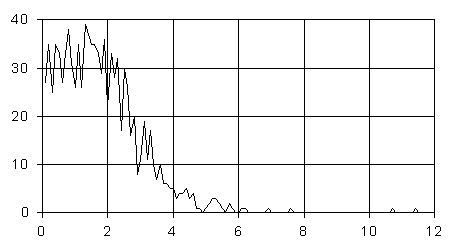
\includegraphics[width=0.8\textwidth]{figures/4_12.jpg}
  \caption{The distribution of problems of the class $G_{HL}$}
  \label{fig:4_12}
\end{figure}

The distribution of the interval lengths $[\alpha,\beta]$ from (4.41) including the solution points $x^*$ corresponding to the problems from the first set is presented in Fig. \ref{fig:4_11}. Fig. \ref{fig:4_12} demonstrates a similar distribution for the problems of the second set. In these figures, the values $(\beta=\alpha)/(b-a)$ (in percentage) are plotted against the abscissa axes while the numbers of problems in the corresponding sets are plotted against the ordinate ones. In order to obtain the discussed estimates, the lengths of the intervals $[\alpha,\beta]$ corresponding to the respective functions were determined by a numerical method.

More detailed information on the number of problems (in either of two sets) featured by a small (less than 0.1\%) measure of the interval $[\alpha,\beta]$ is presented below.

\begin{table}
  \caption{The number of problems with a small measure of the interval $[\alpha,\beta]$}
\begin{center}
  \label{tab4:exp_results2}
  \begin{tabular}{cccccccccc}
    \hline
     & 0.01\% & 0.02\% & 0.03\% & 0.04\% & 0.05\% & 0.06\% & 0.07\% & 0.08\% & 0.09\% \\ \hline
    $G_{SH}$ & 0 & 1 & 2 & 1 & 0 & 0 & 1 & 1 & 1  \\ 
    $G_{HL}$ & 3 & 6 & 2 & 3 & 5 & 1 & 2 & 1 & 2 \\ \hline
  \end{tabular}
\end{center}
\end{table}

As follows from the figures and Table \ref{tab4:exp_results2}, the problems from the second set produced by generator $G_{HL}$ are characterized in general by a narrower feasible vicinity of the solution point $x^*$.

The constraint functions $g_\nu( x ),\: 1 \le\nu\le 5$, and the objective function $\varphi (x)$ for a problem from the class $G_{HP}$ are plotted in Fig. \ref{fig:4_13} as an example. The feasible domains which are formed by the separate constraints are marked on the abscissa axis. The whole feasible domain of the problem (the intersection of all feasible domains of the constraints) is shown along with the graph of the objective function.

\begin{figure}[ht]
  \centering
  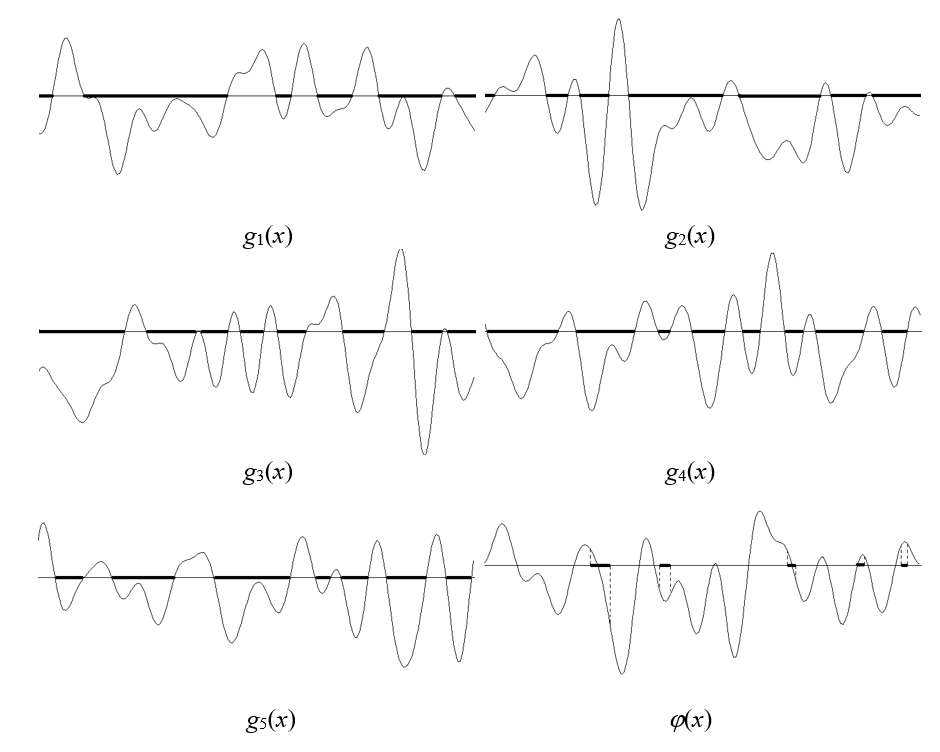
\includegraphics[width=0.8\textwidth]{figures/4_13.png}
  \caption{Function plots of a test problem from the class $G_{HL}$}
  \label{fig:4_13}
\end{figure}

The experiments have been carried out for the algorithms described above with the fixed constraints’ check order and with the adaptive one (FCOM and ACOM, respectively). The parameters $r_\nu, 1\le\nu\le 5$, from (4.17) were defined by the expressions
\begin{displaymath}
  r_\nu = \left\{
  \begin{array}{lr}
    \gamma, & k_\nu < 20\\
    2, & k_\nu \ge 20
  \end{array}
  \right.,
\end{displaymath}
where $k_\nu$ is the number of the calculated values of the function $g_\nu$ (i.e., the cardinality of the set $I_\nu$). In the experiments, the values $\gamma=20,\: \epsilon = 0.001$, and the reserves $\epsilon_\nu=0.1,\: 1\le\nu\le 5$, were set for the set produced by the generator $G_{SH}$. For the problems from the second set (generator $G_{HL}$ ) the values  $\gamma=10,\: \epsilon = 0.0001$, and the reserves $\epsilon_\nu=0.001,\: 1\le\nu\le 5$, were used.

\begin{figure}[ht]
  \centering
  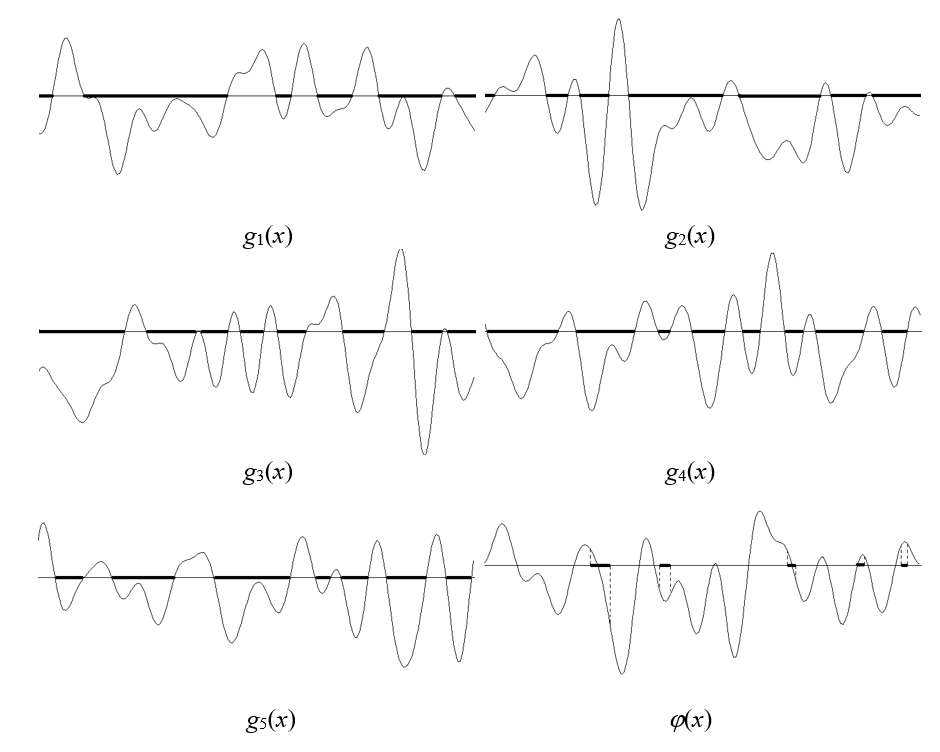
\includegraphics[width=0.8\textwidth]{figures/4_13.png}
  \caption{Operational characteristics for the class $G_{SH}$}
  \label{fig:4_14}
\end{figure}

\begin{figure}[ht]
  \centering
  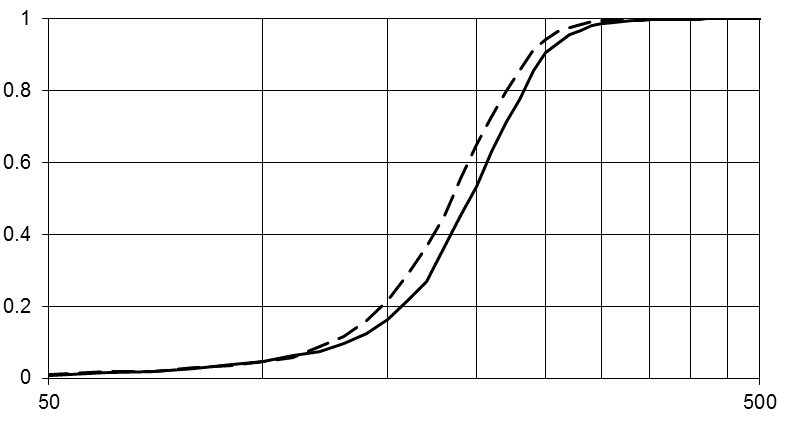
\includegraphics[width=0.8\textwidth]{figures/4_15.png}
  \caption{Operational characteristics for the class $G_{HL}$}
  \label{fig:4_15}
\end{figure}

The operational characteristics for both the methods obtained on the sets produced by generators $G_{SH}$ and $G_{HL}$ are presented in figures \ref{fig:4_14} and \ref{fig:4_15}, respectively. The lower (solid) curves correspond to FCOM while the upper (dashed) ones --- to ACOM. These positions of the curves demonstrate that the algorithm with the adaptive check order provides in average faster obtaining the estimates falling into given vicinity of the solution than the algorithm with the fixed checking order.

\begin{figure}[ht]
  \centering
  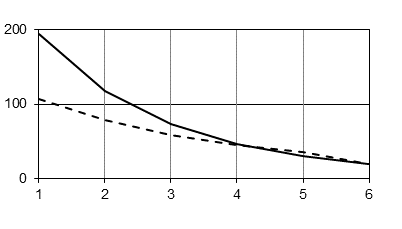
\includegraphics[width=0.8\textwidth]{figures/4_16.png}
  \caption{Average number of function values computations for the class $G_{SH}$}
  \label{fig:4_16}
\end{figure}

\begin{figure}[ht]
  \centering
  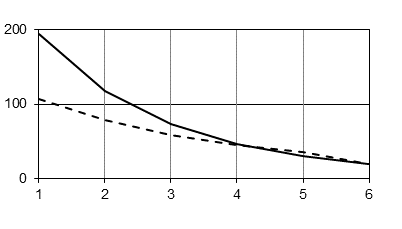
\includegraphics[width=0.8\textwidth]{figures/4_17.png}
  \caption{Average number of function values computations for the class $G_{HL}$}
  \label{fig:4_17}
\end{figure}

Moreover, the trials executed according to the rules of ACOM appear to be much less computation costly (in average) than the ones executed by FCOM. This fact is illustrated in figures 4.16 and 4.17, where the average number of computations of the function values executed by FCOM and ACOM for given sets are presented. Fig. 4.16 corresponds to the generator $G_{SH}$ while Fig. 4.17 shows the results for the generator $G_{HL}$. In both figures the function indices are plotted on the abscissa axes. The estimates of the average numbers of the computations of these function values during the trials’ execution are marked on the plot axes. The solid lines in the figures connect the points of the estimates corresponding to FCOM while the dashed ones connect the points of estimates corresponding to ACOM. The presented data confirm that introducing the adaptive constraints’ check order can reduce the total number of the computations essentially.

\section{Parallel computations for the multiextremal optimization problems with nonlinear constraints}
\subsection{Asynchronous parallel index algorithm}
In this subsection the asynchronous parallel index algorithm with $p>1$ parallel processors for solving the problem \eqref{ex4:problem} will be presented.

The first $p$ trial points are selected at the internal points of the interval $[a,b]$ arbitrarily. Each processor starts the trials execution at the corresponding points. After completing the $k$-th trial, when the points $x^{k+1},\dots, x^{k+p - 1}$ have already been selected but the trial results at these points are not obtained yet, the point of the next trial $x^{k+p}$ is selected according to the following rules.

\emph{Rule 1.} Renumber the points of the preceding trials $x^1,\dots,x^k$ by the subscripts in the increasing order of the coordinate values, i.e.,
\begin{equation}
  \label{eq4:par_search_data}
  a=x_0<x_1<\dots x_i<\dots<x_{k+p-1}<x_{k+p}=b,
\end{equation}
the points $x_0=a$ and $x_{k + p}=b$ are included into series \eqref{eq4:par_search_data} additionally for the convenience of the future notation.

\emph{Rule 2.} Determine the set $I$ of the points $x_i,\: 1\le i<k+p$, such that the trials at these points have not been completed yet.

\emph{Rule 3.} Juxtapose to each point $x_i,\: 1\le i<k+p$, from series \eqref{eq4:par_search_data} such that $x_i\not\in I$ the
index $\nu=\nu(x_i)$ and the value $z_i=g_\nu(x_i )$ calculated at this point (the values $z_0$ and $z_{k + p}$ are not determined).

\emph{Rule 4.} Construct the sets
\begin{equation}
  I_\nu=\{i:1\le i<k+p, \nu=\nu(x_i),x_i\not\in I\},\:1\le\nu\le m+1,
\end{equation}
including the subscripts of all points $x_i ,1\le i<k+p$, with the same index, in which the trials are completed at the moment. The boundary points $x_0=a$ and $x_{k + 1}=b$ are considered as the points with the zero indices. The additional set $I_0=\{0,k+1\}$ is associated with these points.

Find the maximum value of the index
\begin{equation}
  M=\max\{\nu=\nu(x_i),x_i\not\in I,1\le i \le k\}.
\end{equation}

\emph{Rule 5.} Compute current estimates
\begin{equation}
  \label{eq4:lip_est_par}
  \mu = \max\left\{ \frac{\left|z_i-z_j\right|}{ x_i - x_j }, \; i,j \in I_\nu, \; i>j \right\},
\end{equation}
for the unknown Lipschitz constants $L_\nu$ of the functions $g_\nu,\: 1\le\nu\le m+1$. If the set $I_\nu$ includes less than two elements or if $\mu_\nu$ from \eqref{eq4:lip_est_par} appears to be equal to zero, to set $\mu_\nu=1$.

\emph{Rule 6.} For all nonempty sets $I_\nu,\: 1\le\nu\le m+1$ calculate the estimates
\begin{equation}
  \label{eq4:z_const_par}
  z_\nu^\ast = \left\{
  \begin{array}{lr}
    -\epsilon_\nu, & \nu < M,\\
    \min\{ g_\nu(y(x_i): i\in I_\nu \}, & \nu = M.
  \end{array}
  \right.
\end{equation}
where the vector $\epsilon_R=(\epsilon_1 ,\dots, \epsilon_m )$ is a given vector with the non-negative components (\emph{the reserve vector}).

\emph{Rule 7.} Compute the characteristics $R(i)$ for each interval $(x_{i-1}, x_i ),\: x_{i – 1}\not\in I,\: x_i\not\in I, 1\le i\le k+p$ where
\begin{gather}
  R(i)=2\Delta_i-4\frac{z_i-z_\nu^\ast}{r_\nu \mu_\nu}, \; \nu=\nu(x_i)>\nu(x_{i-1}), \nonumber \\
  \label{eq4:characteristic_par}
  R(i)=\Delta_i+\frac{(z_i-z_{i-1})^2}{r_\nu^2 \mu_\nu^2\Delta_i}-2\frac{z_i+z_{i-1}-2z_\nu^\ast}{r_\nu \mu_\nu}, \;  \nu=\nu(x_i)=\nu(x_{i-1}),\\
  R(i)=2\Delta_i-4\frac{z_{i-1}-z_\nu^\ast}{r_\nu \mu_\nu}, \; \nu=\nu(x_{i-1})>\nu(x_i), \nonumber \\
  \Delta_i=x_i - x_{i-1} \nonumber
\end{gather}
where the values $r_\nu>1,\: 1\le\nu\le m+1$ are the algorithm parameters and $\Delta_i=x_i-x_{i-1}$.

\emph{Rule 8.} Select the interval $(x_{t-1},x_t )$ whith the largest characteristic
\begin{equation}
  \label{eq4:MaxR_par}
  R(t)=\max\{R(i):x_{i-1}\not\in I,x_{i}\not\in I,1\le i\le k+p\}.
\end{equation}

\emph{Rule 9.} Execute the next trial at the middle point of the interval $(x_{t-1},x_t )$ if the indices of its boundary points are not the same, i.e.,
\begin{equation}
  \label{eq4:next_point_1_par}
  x^{k+1} = \frac{x_t + x_{t-1}}{2}, \; \nu(x_{t-1}) \neq \nu(x_t).
\end{equation}
Otherwise, accept
\begin{equation}
\label{eq4:next_point_2_par}
x^{k+p} = \frac{x_t+x_{t-1}}{2} - \frac{z_t-z_{t-1}}{2r_\nu\mu_\nu},\; \nu=\nu(x_{t-1})=\nu(x_t).
\end{equation}
as the point of the next trial.

The rules described above can be supplemented with the termination condition
\begin{equation}
\label{eq4:stop_cond_par}
  x_t - x_{t-1}\le\epsilon
\end{equation}
where $t$ from \eqref{eq4:MaxR_par} and $\epsilon>0$ is the predefined accuracy of the search.

\subsection{The convergence conditions of the algorithm}
\begin{theorem}
  \label{th4:convergence_par}
  Assume problem \eqref{eq4:problem} to have a solution $x^*$ and the following conditions to be fulfilled:
  \begin{itemize}
    \item each subdomain $Q_j ,1\le j\le m+1$ from \eqref{eq4:q} is a union of a finite number of positive length segments;
    \item each function $g_j ,1\le j\le m+1$ satisfies Lipschitz condition with the corresponding constant $L_j$;
    \item the components $\epsilon_\nu$ of the reserve vector $\epsilon_R$ satisfy the inequalities
    \begin{equation}
      \label{eq4:reserves_par}
      0<2\epsilon_\nu<L_\nu(\beta-\alpha)
    \end{equation}
    where $\beta-\alpha$ is the length of the interval $[\alpha,\beta]$ belonging to the feasible domain $Q$ from \eqref{eq4:Q_union} and including the point $x^*$ which is the solution of the problem;
    \item beginning from sufficiently large step number $k$, the values $\nu_\nu$ from \eqref{eq4:lip_est_par} corresponding to the nonempty sets $I_\nu$ satisfy the inequalities
    \begin{equation}
      r_\nu\mu_\nu>2L_\nu,\:1\le\nu\le m+1,
    \end{equation}
    where the algorithm parameters $r_\nu>1,\:1\le\nu\le m+1$;
    \item during the parallelization, the inequalities
    \begin{displaymath}
      T^j_{l+1}-T^j_j<T<\infty,1\le j\le p, l>1,
    \end{displaymath}
    are true where $T_l^j$ is the moment of completing the $l$-th trial by the $j$-th processor and the inequality $1<p<P<\infty$ takes place for the number of processors $p$.
  \end{itemize}
  Then:
  \begin{itemize}
    \item the point $x^*$ is a limit one for the sequence ${x^k }$ generated by the described asynchronous algorithm for problem \eqref{eq4:problem} if $\epsilon=0$ in termination condition \eqref{eq4:stop_cond_par};
    \item any limit point $\overline x$ of the sequence $\{x_k \}$ is a solution of the problem \eqref{eq4:problem};
    \item the convergence to the limit point $\overline x$ is bilateral if $\overline x\not=a$ and $\overline x\not=b$.
  \end{itemize}
\end{theorem}

Before the proof of the theorem, let us formulate and prove several auxiliary statements.

\begin{lemma}
  (on the sequence of the shrinking intervals). Assume the conditions of Theorem \ref{th4:convergence_par} to be satisfied. Then for each limit point $x$ of the sequence $\{x_k\}$ there exists an infinite sequence of the intervals
  \begin{equation}
    \{(x_{t-1},x_t):t=t(q^s)\},\:s=1,2,\dots,
  \end{equation}
  satisfying the conditions
  \begin{gather}
    \overline x= \cap_{s=1}^\infty[x_{t-1},x_t], \\
    \lim_{p\to\infty}\Delta_t=0, \\
    R(t(q^s))>0,\:s=1,2,\dots, \\
    \lim_{p\to\infty}R(t(q^s))=0,
  \end{gather}
  where $q^1<q^2<\dots;\:R(t),\:\Delta_t$, and $t$ are from rules \eqref{eq4:characteristic_par} and \eqref{eq4:MaxR_par}, correspondingly.
\end{lemma}

\begin{proof}
  Since $\overline x$ is a limit point, there exists a sequence of the trial numbers $q^1,q^2,\dots$ satisfying the conditions
  \begin{equation}
    x^{q+1},\overline x\in[x_{t-1},x_t], t=t(q),q\in\{q^p\},p=1,2,\dots.
  \end{equation}
  These conditions reflect the fact that the point of the $(q+1)$-th trial falls into the interval $[x_{t-1},x_t]$ containing the point $\overline x$ at the step $q$, i.e., $t=t(q)$.

  It follows from this condition, from the rules of the next trial point selection \eqref{eq4:next_point_1_par} and \eqref{eq4:next_point_2_par}, and from the estimate of the value $\mu_\nu$ from \eqref{eq4:lip_est_par}, that
  \begin{equation}
    \label{eq4:4_60}
    \max\{x_t-x^{q+1},x^{q+1}-x_{t-1}\}\le\gamma \Delta_t,
  \end{equation}
  where $\gamma=(r+1)/2r<1$ and
  \begin{equation}
    r=\min\{r_\nu:1\le\nu\le m+1\}>1.
  \end{equation}
  Then, the property (4.56) is a consequence of inequality \eqref{eq4:4_60}.

  At every step $k\ge 1$ there exists an interval $(x_{i-1},x_i), \:i=i(k)$, at one of the ends of which the value $z^*_\omega$ from \eqref{eq4:z_const_par} is achieved. This value corresponds to the index $\omega$ defined (when $\omega<m$) by the conditions $I_\omega\not= \varnothing,\: I_{\omega+1} =  \varnothing$. If $I_{m+1}= \varnothing$, the index $\omega=m+1$. If at that $\nu(x_{i -1} )\not = \nu(x_i )$, then according (4.47) and (4.50), $R(i)=2\Delta_i>0$. In the case when $\nu(x_{i -1} )= \nu(x_i )=\omega$, the estimate
  \begin{displaymath}
    \max(z_{i-1}, z_i)-z^*_\omega\le\mu\Delta_i
  \end{displaymath}
  follows from \eqref{eq4:lip_est_par} and, along with \eqref{eq4:characteristic_par}, gives the estimate
  \begin{displaymath}
    R(i)=\Delta_i\left(1-\frac{\max(z_{i-1},z_i)-z^*_\omega}{r_\omega\mu_\omega\Delta_i}\right)\ge (1-r^{-1})\Delta_i,
  \end{displaymath}
  where $r$ is from (4.61). Thus, at any search step $k\ge 1$ there exists an interval having a strictly positive characteristic. Hence, taking into account the rules of selection of the interval with the greatest characteristic \eqref{eq4:MaxR_par}, one can conclude that the intervals from system (4.54) should also have the positive characteristics since these ones undergo splitting up by the trial points falling into these intervals. Consequently, conditions (4.57) hold.

  It follows from the trial execution rules and condition (4.35) that for $\nu(x_i )\le m$ the values $z_i$ assigned to the points $x_i$ from \eqref{eq4:par_search_data} are positive. Therefore, according to \eqref{eq4:z_const_par},
  \begin{displaymath}
    z_i=g_\nu(x_i)\ge z^*_nu,\:1\le\nu=\nu(x_i)\le m+1,\: 0\le i\le k.
  \end{displaymath}
    Now from the rules \eqref{eq4:characteristic_par} for the characteristics and the limit (4.56), taking into account the condition \eqref{eq4:lip_condition} of Lipschitzness of the functions and inequality (4.57), one can derive out the truth of statement (4.58).
\end{proof}
\begin{lemma}
  \label{lm4:2}
  (on the existence of a feasible point). Assume the conditions of Theorem \ref{th4:convergence_par} to be fulfilled. Then, there exists the trial index $h\ge 1$, for which
  \begin{equation}
    \label{eq4:62}
    \nu(x^h)=m+1.
  \end{equation}
\end{lemma}
\begin{proof}
  Let us assume the opposite and consider the interval $[x_{t-1},x_t]$ including the problem solution $x^*$ from \eqref{eq4:problem} at the step $k$, i.e., $t=t(k)$. Since we have assumed the equality \eqref{eq4:62} not to take place and, consequently, the sequence $\{x^k\}$ does not include the points from the feasible domain $Q$, the interval $[\alpha,\beta]$ from (4.52) should satisfy the conditions
  \begin{equation}
    \label{eq4:63}
    x^*\in [\alpha,\beta]\subset[x_{t-1}, x_t].
  \end{equation}
  Then, from this condition as well as from the Lipschitz properties of the problem functions the relations
  \begin{gather}
    z_{t-1}\le L_\nu(\alpha - x_{t-1})\le L_\nu\Delta_t-L_\nu(\beta-\alpha),\:\nu=\nu(x_{t-1}) \\
    z_t\le L_\nu(x_{t}-\beta)\le L_\nu\Delta_t-L_\nu(\beta-\alpha),\:\nu=\nu(x_{t})
  \end{gather}
  follow. It was taken into account when deriving out of the above relations that
  \begin{displaymath}
    g_\nu(x)\le 0,\: x\in[\alpha,\beta]\subset Q.
  \end{displaymath}
  Analogously, the case $\nu=\nu(x_{t-1})=\nu(x_t)$ corresponds to the inequality
  \begin{equation}
    z_t+z_{t-1}\le L_\nu \Delta_t - L_\nu(\beta-\alpha).
  \end{equation}

  Now, from the characteristic rules \eqref{eq4:characteristic_par}, from inequalities (4.64)–(4.66), and from the inequality
  \begin{displaymath}
    z^*_\nu\ge-\epsilon_\nu
  \end{displaymath}
  resulting from \eqref{eq4:z_const_par} either the estimate
  \begin{displaymath}
    R(t)\ge\Delta_t(1-2L_\nu/r_\nu\mu_\nu)+2(L_\nu(\beta-\alpha)-2\epsilon_\nu)/r_\nu\mu_\nu,
  \end{displaymath}
  or the estimate
  \begin{displaymath}
    R(t)\ge\Delta_t(1-2L_\nu/r_\nu\mu_\nu)+4(L_\nu(\beta-\alpha)-2\epsilon_\nu)/r_\nu\mu_\nu,
  \end{displaymath}
  is true. Taking into account the third condition of Theorem \ref{th4:convergence_par} and the fourth one, in both cases we get the inequality
  \begin{equation}
    \label{eq4:67}
    R(t(k))>0
  \end{equation}
  which holds for sufficiently large step numbers $k$.

  From (4.58), \eqref{eq4:67}, and from the rule (4.48) determining the choice of the interval for the next trial point, the inevitability of carrying out a trial in the interval $[x_{t-1},x_t]$ from (4.63) follows. Consequently, the interval $[x_{t-1},x_t]$ will be divided into two subintervals. After that, at least one of those will include the point $x^*$. The repetition of this division generates (with $k\to\infty$) an infinite sequence of the subintervals shrinking to the point $x^*$ . In other words, if the third condition of Theorem \ref{th4:convergence_par} and the fourth one are satisfied, $x^*$ is the limit point of the sequence ${x^k}$.

  Since the coincidence $x^*$ with one of the trial points means (4.62) to hold, then it remains to consider the case when $x^*\in(x_{t- 1} ,x_t ),\: t=t(k)$ for any $k\ge 1$. Here, because of the first condition of Theorem \ref{th4:convergence_par} and the definition (4.31) either $[x_{t-1},x^*]\in Q$ or $[x^* ,x_t]\in Q$ if the number $k$ is sufficiently large. In this case, either $\nu(x_{t-1})=m+1$ or $\nu (x_t )=m+1.$
\end{proof}

\begin{lemma}
  \label{lm4:3}
  on the feasibility of any limit point). Assume the conditions of Theorem \ref{th4:convergence_par} to be met. Then any limit point $\overline x$ of the sequence $\{x_k\}$ is feasible, i.e.,
  \begin{equation}
    \label{eq4:68}
    \nu(\overline x)=m+1
  \end{equation}
\end{lemma}

\begin{proof}
  Let us assume the opposite. According to (4.55) and (4.56),
  \begin{displaymath}
    \overline x = \lim_{s\to\infty}x_{t-1}=\lim_{s\to\infty}x_t, t=t(x^s).
  \end{displaymath}
  where q s is from (4.57) Therefore, it follows from the assumption $x\in Q$ that there exists such large number $S>1$ and such small subinterval
  \begin{equation}
    \label{eq4:69}
    (u,w)\subset[a,b]\setminus Q,
  \end{equation}
  that
  \begin{equation}
    [x_{t-1},x_t]\subset(u,w),\:t=t(q^s),\:s\ge S.
  \end{equation}

  Let us assign to $Q_j, 1\le j\le m$, from (4.30) their open complements $D_j=[a,b]\setminus Q_j$ consisting of finite number of the open intervals with the positive length (as a consequence of the first condition of Theorem \ref{th4:convergence_par}). For these complements
  \begin{equation}
    g_j(x)>0,x\in D_j,\:1\le j\le m.
  \end{equation}

  It follows from \eqref{eq4:69} that there exist such subsets of indices $M,N\subset\{1,2,\dots,m\}$ that
  \begin{equation}
    (u,\overline x]\subset \cap_{j\in M}D_j,\:[\overline x,w)\subset \cap_{j\in N},
  \end{equation}
  where $(u,w)$ is an open interval from \eqref{eq4:69}.

  According to the trial execution rules and to conditions (4.35) and (4.72), for any interval from (4.70) the relations
  \begin{displaymath}
    \omega_1=\nu(x_{t-1})\in M,\: \omega_2=\nu(x_t)\in N,\:t=t(q^s),
  \end{displaymath}
  hold where $1\le \omega_1,\: \omega_2\le m$. Moreover, according to the rules (4.39) and (4.40) defining the constraints’ check order at trial points,
  \begin{displaymath}
    \nu(x_{t-1}),\:\nu(x_t)\in\{\omega_1,\omega_2\},\: t=t(q^{p+1}).
  \end{displaymath}
  In other words, for sufficiently large number $s>1$ the indices assigned to the boundary points of the considered system of intervals $[x_{t-1},x_t],\: t=t(q^s ): s\ge S$ can take the values from the set $\{\omega_1,\omega_2\}$ only.

  Now, from (4.46), (4.74), and (4.57) one can conclude that if the point $x$ is not a feasible one, it cannot be a limit point of the sequence $\{x^k\}$, i.e., for any limit point $x$ the condition \eqref{eq4:68} is true.
\end{proof}

\begin{proof} (of Theorem \ref{th4:convergence_par}).

  I. Let us prove the first assertion of Theorem \ref{th4:convergence_par} based on Lemma \ref{lm4:2} and Lemma \ref{lm4:3}, i.e., that the point $x^*$ from \eqref{eq4:problem} is the limit point. Let us assume the opposite and consider two  possible cases. Assume $[x_{t-1},x_t],\: t=t(k)$ to be an interval including the point $x^*$ at the step $k$. Consider the condition
  \begin{equation}
    \label{eq4:75}
    \max\{\nu(x_{t-1}),\nu(x_t)\}=m+1
  \end{equation}
  for the indices of the boundary points of the given interval and assume that this condition is not satisfied for sufficiently large $k$. In this case, inclusions \eqref{eq4:63} should take place. This situation has been already considered in Lemma \ref{lm4:2}, where its incompatibility with the assumption of the point $x^*$ is not the limit point has been demonstrated.

  So, it remains to consider the case when condition \eqref{eq4:75} is fulfilled for some subsequence of the step numbers $k$. Then, the relations
  \begin{gather}
    z_{t-1}\le g_\nu(x^*)+L_\nu(x^*-x_{t-1}),\: \nu=\nu(x_{t-1}), \nonumber \\
    z_t\le g_\nu(x^*)+L_\nu(x_t-x^*),\: \nu=\nu(x_t), \nonumber
  \end{gather}
  follow from \eqref{eq4:lip_condition} and the equality $g_{m+1}(x^*)=\varphi(x^*)$ and the inequality
  \begin{displaymath}
    z_t+z_{t-1}\le 2\varphi(x^*)+L_{m+1}\Delta_t,
  \end{displaymath}
  correspond to the case
  \begin{equation}
    \label{eq4:76}
    \nu(x_{t-1})=\nu(x_t)=m+1,
  \end{equation}

  From (4.47) taking into account \eqref{eq4:75} and the inequality $z_{m + 1}\ge \varphi(x)$ resulting from (4.46), one can derive the estimate
  \begin{equation}
    \label{eq4:77}
    R(t)\ge \gamma\Delta_t(1-2L_{m+1}/(r_{m+1}\mu_{m+1}))
  \end{equation}
  where the coefficient $\gamma=1$ in the case when equality \eqref{eq4:76} holds. Otherwise, $\gamma= 2$.

  Now, it follows from \eqref{eq4:77} and from the fourth condition of Theorem \ref{th4:convergence_par} that inequality \eqref{eq4:67} holds for some subsequence of $k$ that, as it has been already discussed above, leads to the contradiction to the assumption of the non-limit character of the point $x^*$.

  II. Let us demonstrate that any limit point $\overline x$ of the sequence $\{x^k\}$ generated by ACOM is a solution of the problem \eqref{eq4:problem} under the conditions of the theorem. Since the point $x^*$ from \eqref{eq4:problem} is a limit one, then, according to (4.46),
  \begin{equation}
    \label{eq4:78}
    \lim_{p\to\infty}z^*_{m+1}=\varphi(x^*).
  \end{equation}

  Let $x\not=x^*$ is another limit point of the sequence $\{x^k\}$ being a feasible one according to \eqref{eq4:68}. Then, for the characteristic of the interval $[x_{j-1},x_j]$ including the point $\overline x$ at the step $k$, because of Lipschitz condition \eqref{eq4:lip_condition}, (4.45), (4.47), (4.56), and \eqref{eq4:78} the relation
  \begin{displaymath}
    \lim_{k\to\infty}R(j(k))\le-4(\varphi(\overline x)-\varphi(x^*))/(r_{m+1}L_{m+1}).
  \end{displaymath}
  holds.

  If $\varphi(x)>\varphi(x^*)$ the characteristic of the interval $[x_{j-1},x_j]$ including the point $\overline x$ will become negative starting from some step that contradicts to property (4.57), which should be fulfilled for any limit point. Consequently, the equality $\varphi(x)=\varphi(x^*)$  is true.

  Theorem is proved.
\end{proof}

\section*{A brief conclusion}
Constrained global optimization problems are under consideration. The method of penalty functions is one of the most popular numerical methods for solving the problems of this kind. Nevertheless, the method of penalty functions has a number of disadvantages. A new method for reduction of a constrained problem to an unconstrained one, so called \emph{index method}, has been considered in this chapter. This method, unlike the classical penalty function one, allows avoiding the problem of the parameter selection (like the penalty coefficients for the constraints). It is also allows solving the problems with partially defined objective function and constraints. This is quite natural for many applied problems, especially, in the optimal design of technical systems, because if some conditions of operation are not met, then some other characteristics of the system performance may not be defined.

The issues of convergence acceleration of the index method have been considered also. Two approaches for the convergence acceleration have been proposed. The first of them is based on concept of $\varepsilon$-reserved solution to the constrained problem. The role of $\varepsilon$-reserved solution in constrained global optimization problems is somewhat similar to the regularity requirements in classical nonlinear programming problems. The second approach is based on adaptive order of checking for constraints. In the index method, every iteration performed at the corresponding point of the search domain includes checking for constraints of the problem at this point. When a violation is discovered for the first time, the current iteration is stopped, and the next iteration is initiated. However, in Lipschitz optimization problems a constraint violated at a point of the search domain is also violated in a certain neighborhood of this point. In this case, to reduce the number of checks, it is expedient to begin iterations in the neighborhood of this point with checking for the violated constraint. Thus, the iteration can be completed at a lower cost.

For all proposed algorithms, the results of numerical experiments are presented. The results confirm the theoretical statements about convergence acceleration.
\begin{thebibliography}{99.}
  \bibitem{stronginMarkin1986} Strongin, R.G., Markin, D.L.: Minimization of multiextremal functions under nonconvex constraints. Cybernetics \textbf{22}(4), 486---493 (1986)
  \bibitem{stronginMarkin1987} Markin, D. L., Strongin, R. G.: A Method for Solving Multi-Extremal Problems with Non-Convex Constraints, That Uses a Priori Information about Estimates of the Optimum. Comput. Maths. Math. Phys. \textbf{27}(1), 33---39 (1987)
  \bibitem{strongin1992} Strongin, R.G.: Algorithms for multi-extremal mathematical programming problems employing the set of joint space-filling curves. Journal of Global Optimization \textbf{2}(4), 357--378 (1992)
  \bibitem{stronginSergeyev2000} Strongin, R.G., Sergeyev, Y.D.: AGlobal Optimization with Non-Convex Constraints. Sequential and Parallel Algorithms. Kluwer Academic Publishers, Dordrecht (2000)
  \bibitem{SergeyevFamularoPugliese2001} Sergeyev Ya.D., Famularo D., Pugliese P.: Index Branch-and-Bound Algorithm for Lipschitz univariate global optimization with multiextremal constraints. Journal of Global Optimization \textbf{21}(3), 317---341 (2001)
  \bibitem{barkalovStrongin2002} Barkalov, K.A., Strongin, R.G.: A global optimization technique with an adaptive order of checking for constraints. Comput. Maths. Math. Phys. \textbf{42}(9), 1289---1300 (2002)
  \bibitem{SergeyevFamularoPugliese2003} Sergeyev Ya.D., Pugliese P., Famularo D.: Index information algorithm with local tuning for solving multidimensional global optimization problems with multiextremal constraints. Mathematical Programming \textbf{96}(3), 489---512. (2003)
  \bibitem{sergeyev2006} Sergeyev Ya.D.: Univariate global optimization with multiextremal non-differentiable constraints without penalty functions. Computational Optimization and Applications \textbf{34}(2), 229---248 (2006)
  \bibitem{sergeyevKhalafKvasov2007} Sergeyev, Y.D., Khalaf, F.M.H., Kvasov, D.E.: Univariate algorithms for solving global optimization problems with multiextremal non-differentiable constraints. In: A. T\"orn, J. ä ilinskas (eds.) Models and Algorithms for Global Optimization, Springer, 123---140 (2007)
  \bibitem{sergeyevKvasovKhalaf2007} Sergeyev Ya.D., Kvasov D.E., Khalaf F.M.H.: A one-dimensional local tuning algorithm for solving GO problems with partially defined constraints. Optimization Letters \textbf{1}(1), 85---99 (2007)
\end{thebibliography}
%\end{document}
